\section{Design For Manufacture And Assembly}

Currently, our idea for making the lock is having keypad in the front and with a camera or with a fingerprint scanner at the top of the lock. Inside the lock, we have an ESP32-C3 that will connect to the wifi and the server. For now, there is only the front side of the lock drawn. We will also have the back side of the lock drawn next. Our design below is a non functioning prototype that is meant for aesthetics.

% Information about side-to-side figures:
% https://tex.stackexchange.com/questions/37581/latex-figures-side-by-side
\begin{figure}[htbp]
    \centering
    \begin{subfigure}[b]{0.48\textwidth}
        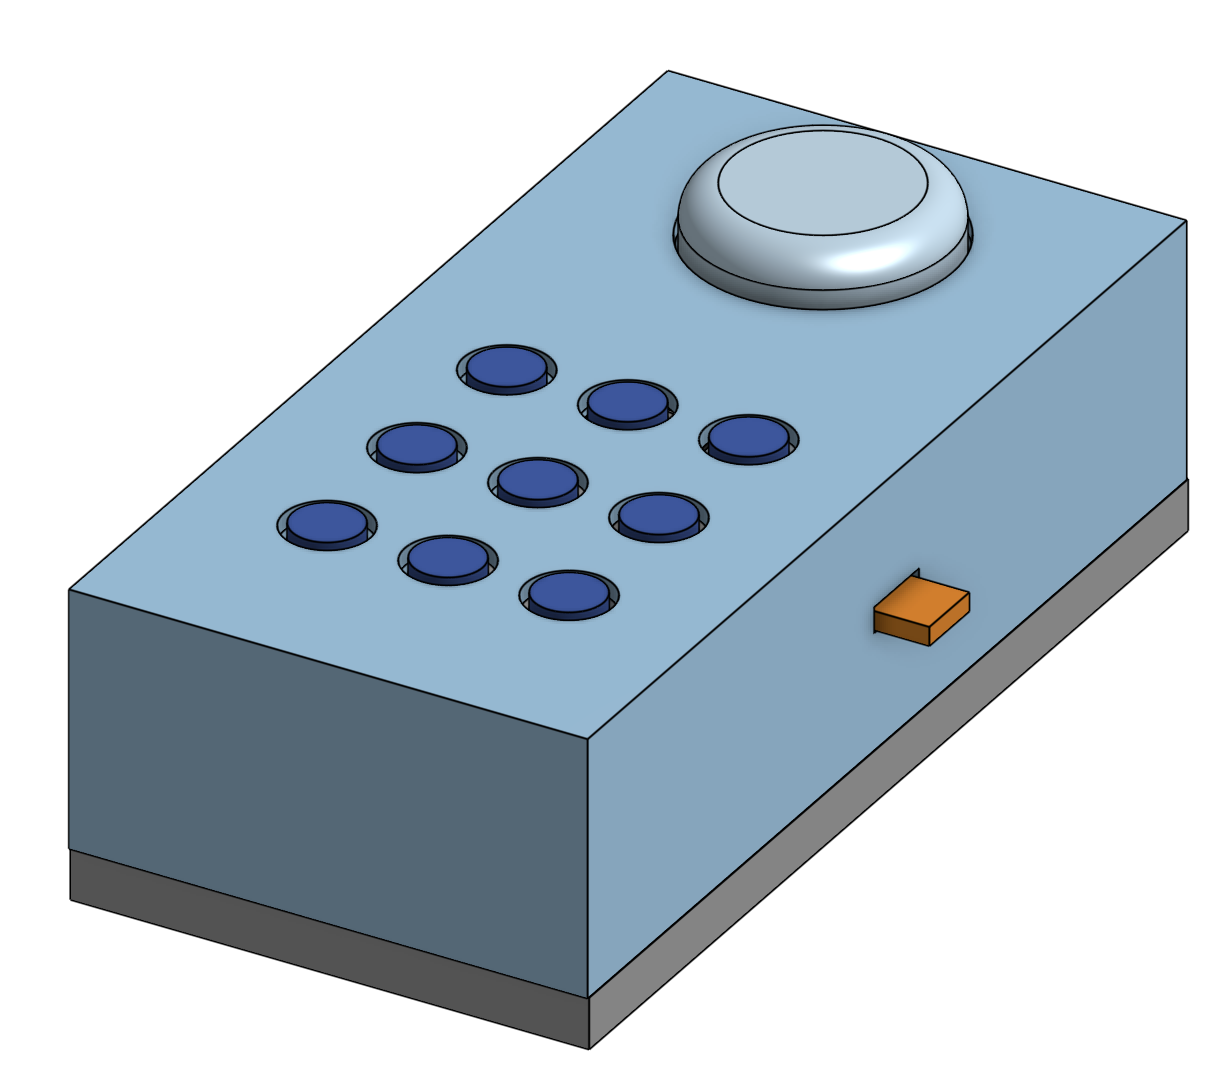
\includegraphics[width=\textwidth]{./img/isoView.png}
        \caption{Isometric View}
        \label{fig:isoView}
    \end{subfigure}
    \hfill
    \begin{subfigure}[b]{0.48\textwidth}
        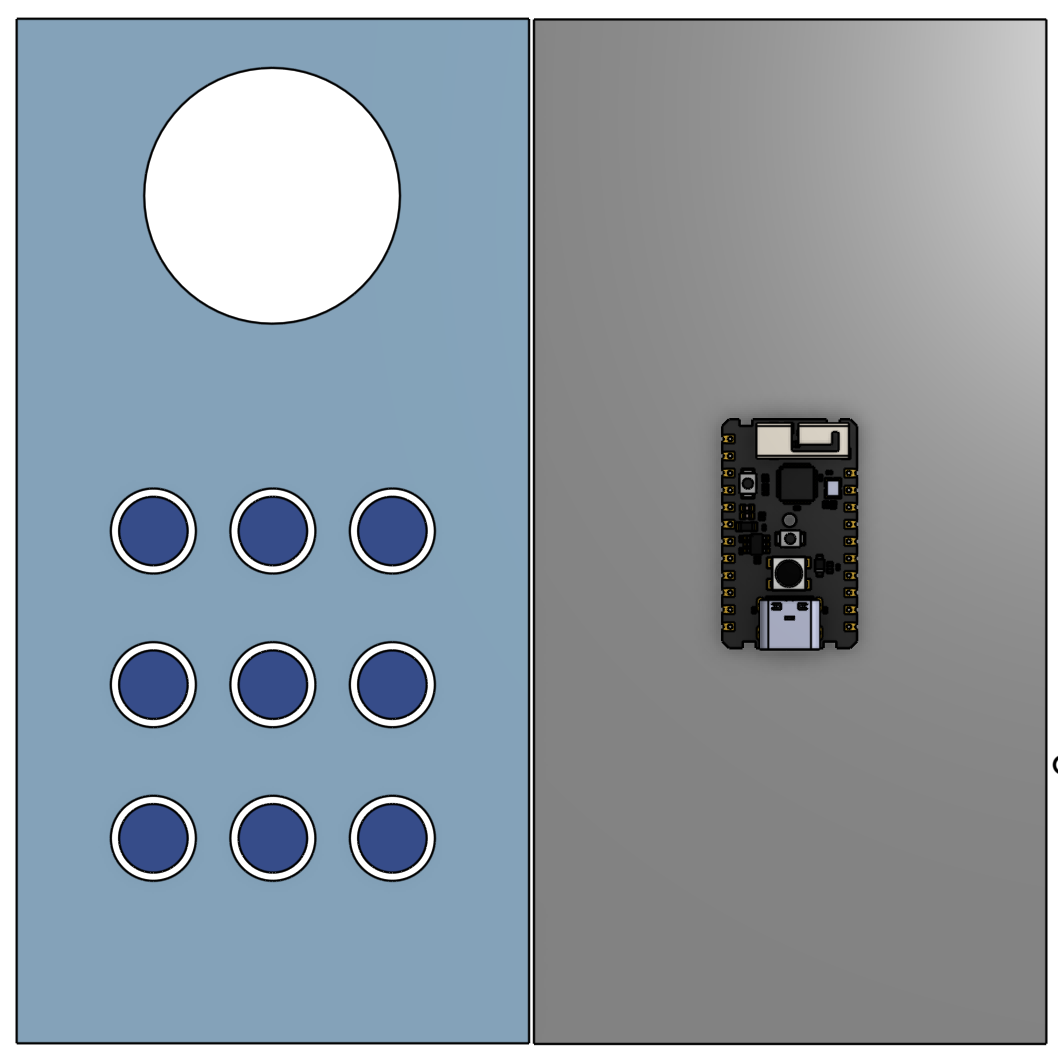
\includegraphics[width=\textwidth]{./img/topView.png}
        \caption{Top View}
        \label{fig:topView}
    \end{subfigure}
    \caption{First lock design}
\end{figure}

The prototype can also be updated in the future, meaning that this will not be the final prototype that we will be building. We will look over the costs and potential flaws that is in our current model.

